\documentclass[top=2cm, bottom=2cm, outer=0cm, inner=0cm]{beamer}
\usetheme{Boadilla}

\usepackage{tikz}
\usepackage{listings}
\usepackage{underscore}
\usepackage[bookmarks=true]{hyperref}
\usepackage[utf8]{inputenc}
\usepackage[english]{babel}
\usepackage{pgfgantt}
\usepackage{CJKutf8}
\hypersetup{
    bookmarks=false,    % show bookmarks bar?
    pdftitle={Software Requirement Specification},    % title
    pdfauthor={Jean-Philippe Eisenbarth},                     % author
    pdfsubject={TeX and LaTeX},                        % subject of the document
    pdfkeywords={TeX, LaTeX, graphics, images}, % list of keywords
    colorlinks=true,       % false: boxed links; true: colored links
    linkcolor=blue,       % color of internal links
    citecolor=black,       % color of links to bibliography
    filecolor=black,        % color of file links
    urlcolor=purple,        % color of external links
    linktoc=page            % only page is linked
}%
\def\myversion{1.0 }
\date{}
%\title
\usepackage{hyperref}

\begin{document}
\setbeamertemplate{frametitle}[default][center]
\begin{CJK}{UTF8}{bkai}
\begin{frame}%%封面
\tikz[remember picture,overlay] \node[opacity=0.2,inner sep=0pt] at (current page.center){
\includegraphics[width=\paperwidth,height=\paperheight]{background}};
\clearpage
\title{\LARGE LINE_BOT簡報}
\author{組員:黃柏凱、陳識允、范喻成、張哲家}
\institute{元智大學資工系}
\date{2018/6/22}
\titlepage
\end{frame}

\begin{frame}%%設計理念
\tikz[remember picture,overlay] \node[opacity=0.2,inner sep=0pt] at (current page.center){
\includegraphics[width=\paperwidth,height=\paperheight]{background}};
\clearpage
\frametitle{\Huge設計理念}
實作風行的LineBot,根據特定的語句,它會有不同的反
應,我們試著利用python來做出也能在Line上運行的機器人。
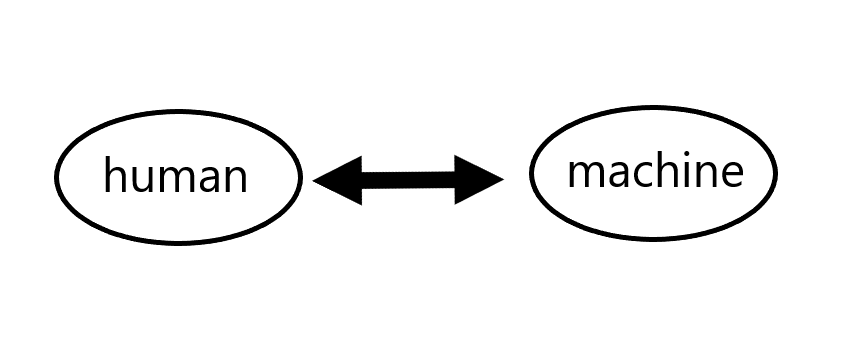
\includegraphics[width=12cm,height=5cm]{relative.png} 
\titlepage
\end{frame}

\begin{frame}%%功能介紹
\tikz[remember picture,overlay] \node[opacity=0.2,inner sep=0pt] at (current page.center){
\includegraphics[width=\paperwidth,height=\paperheight]{background}};
\clearpage
\frametitle{\Huge功能介紹}
\begin{itemize}
\item 語意分析
\pause
\item 翻譯(中翻英、英翻中)
\pause
\item 查詢portal作業
\pause
\item 查詢最新電影
\pause
\item 最新科技新聞
\pause
\item 搜尋縣市天氣
\pause
\item 搜尋youtube音樂
\pause
\item 傳送可愛的狗圖片
\end{itemize}
\titlepage
\end{frame}

\begin{frame}%%語意分析
\tikz[remember picture,overlay] \node[opacity=0.2,inner sep=0pt] at (current page.center){
\includegraphics[width=\paperwidth,height=\paperheight]{background}};
\clearpage
\frametitle{\Huge語意分析}
\vspace{-1cm}
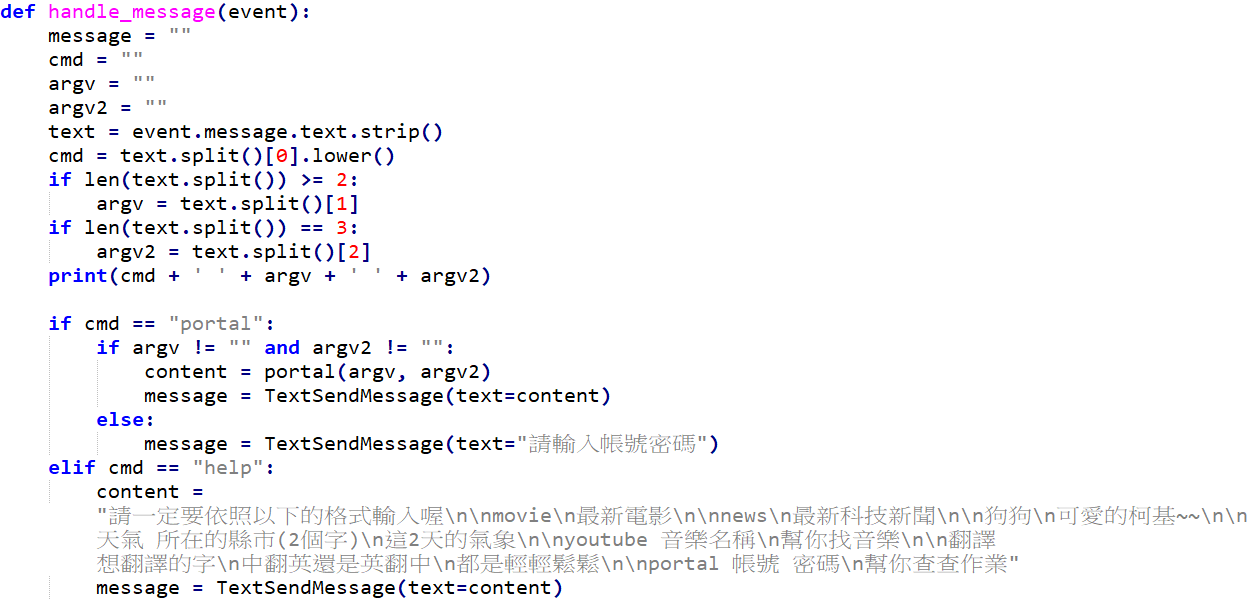
\includegraphics[width=12cm,height=8cm]{recognize.png} 
\titlepage
\end{frame}

\begin{frame}%%翻譯
\tikz[remember picture,overlay] \node[opacity=0.2,inner sep=0pt] at (current page.center){
\includegraphics[width=\paperwidth,height=\paperheight]{background}};
\clearpage
\frametitle{\Huge翻譯}
\vspace{-1cm}
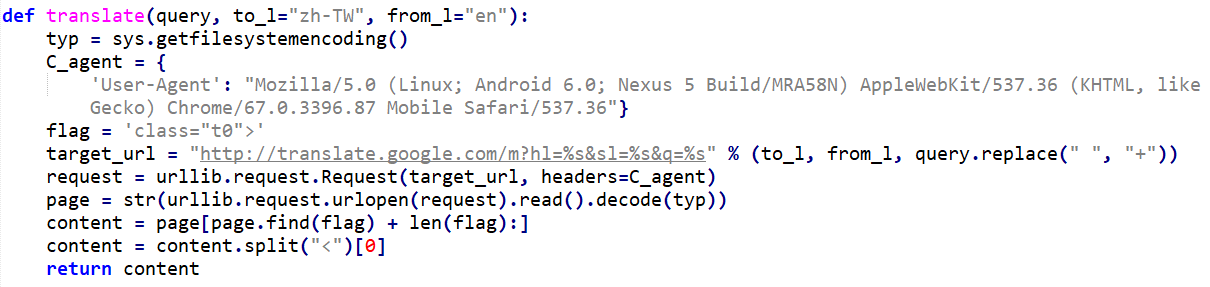
\includegraphics[width=12cm,height=8cm]{translate.png}
\titlepage
\end{frame}

\begin{frame}%%翻譯
\tikz[remember picture,overlay] \node[opacity=0.2,inner sep=0pt] at (current page.center){
\includegraphics[width=\paperwidth,height=\paperheight]{background}};
\clearpage
\frametitle{\Huge翻譯cont.}
\vspace{-1cm}

\includegraphics[width=12cm,height=8cm]{translation.jpg}
\titlepage
\end{frame}

\begin{frame}%%portal
\tikz[remember picture,overlay] \node[opacity=0.2,inner sep=0pt] at (current page.center){
\includegraphics[width=\paperwidth,height=\paperheight]{background}};
\clearpage
\frametitle{\Huge Portal}
\vspace{-1cm}
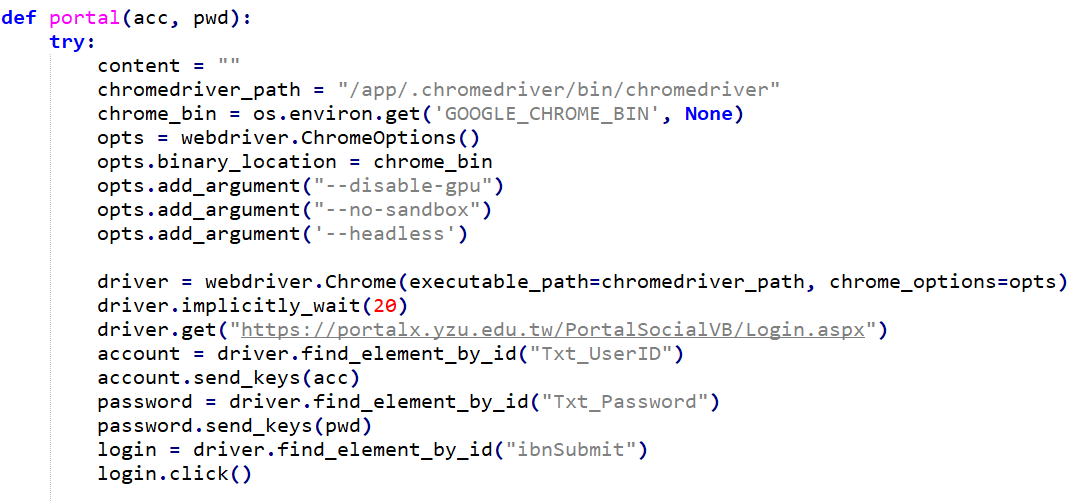
\includegraphics[width=12cm,height=8cm]{portal1.png} 
\titlepage
\end{frame}

\begin{frame}%%portal
\tikz[remember picture,overlay] \node[opacity=0.2,inner sep=0pt] at (current page.center){
\includegraphics[width=\paperwidth,height=\paperheight]{background}};
\clearpage
\frametitle{\Huge Portal cont.}
\vspace{-1cm}
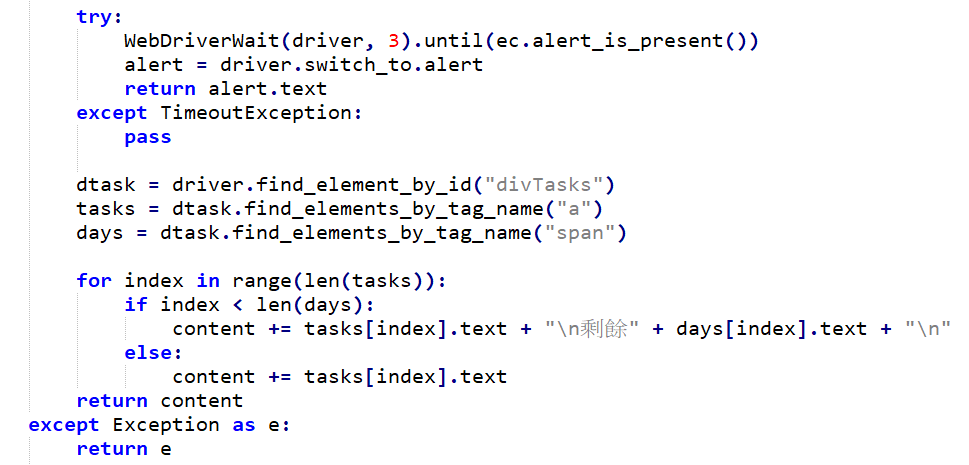
\includegraphics[width=12cm,height=8cm]{portal2.png} 
\titlepage
\end{frame}

\begin{frame}%%portal
\tikz[remember picture,overlay] \node[opacity=0.2,inner sep=0pt] at (current page.center){
\includegraphics[width=\paperwidth,height=\paperheight]{background}};
\clearpage
\frametitle{\Huge Portal cont.}
\vspace{-1cm}
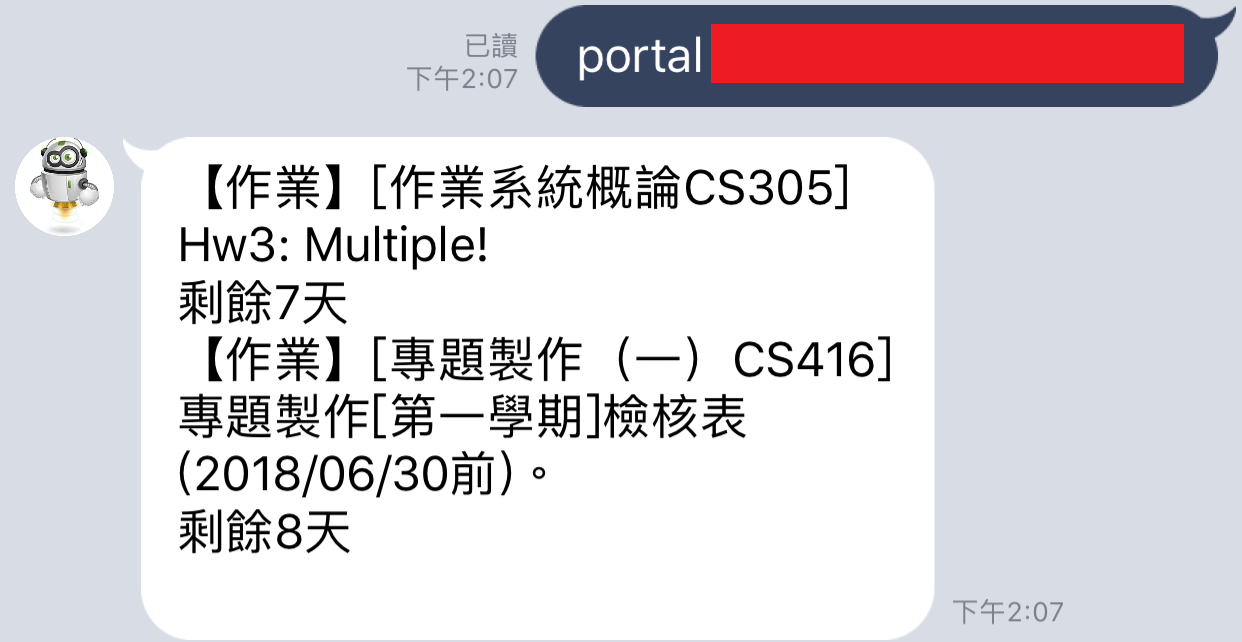
\includegraphics[width=12cm,height=8cm]{portal.jpg} 
\titlepage
\end{frame}

\begin{frame}%%電影
\tikz[remember picture,overlay] \node[opacity=0.2,inner sep=0pt] at (current page.center){
\includegraphics[width=\paperwidth,height=\paperheight]{background}};
\clearpage
\frametitle{\Huge電影}
\vspace{-1cm}
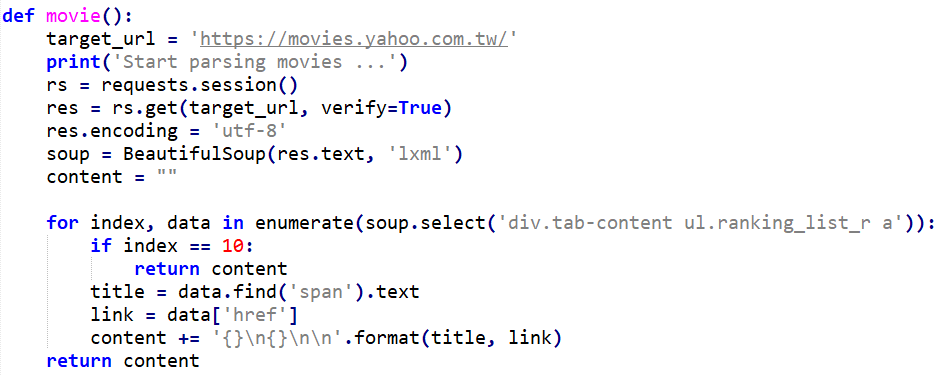
\includegraphics[width=12cm,height=8cm]{movie.png} 
\titlepage
\end{frame}

\begin{frame}%%電影
\tikz[remember picture,overlay] \node[opacity=0.2,inner sep=0pt] at (current page.center){
\includegraphics[width=\paperwidth,height=\paperheight]{background}};
\clearpage
\frametitle{\Huge電影 cont.}
\vspace{-1cm}

\includegraphics[width=12cm,height=8cm]{movie.jpg} 
\titlepage
\end{frame}

\begin{frame}%%新聞
\tikz[remember picture,overlay] \node[opacity=0.2,inner sep=0pt] at (current page.center){
\includegraphics[width=\paperwidth,height=\paperheight]{background}};
\clearpage
\frametitle{\Huge新聞}
\vspace{-1cm}
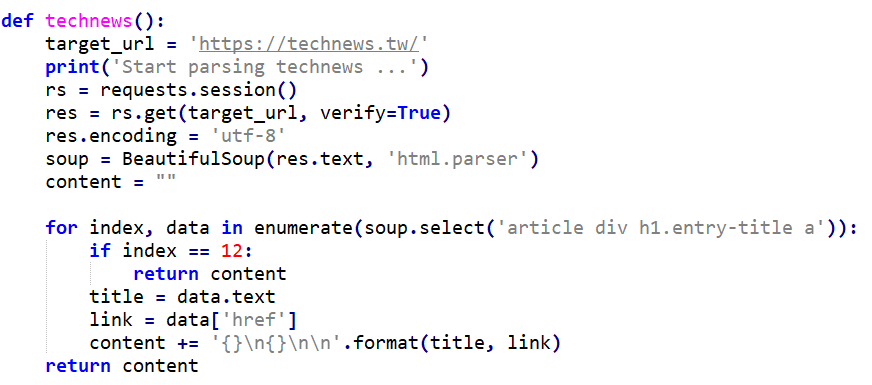
\includegraphics[width=12cm,height=8cm]{technews.png} 
\titlepage
\end{frame}

\begin{frame}%%新聞
\tikz[remember picture,overlay] \node[opacity=0.2,inner sep=0pt] at (current page.center){
\includegraphics[width=\paperwidth,height=\paperheight]{background}};
\clearpage
\frametitle{\Huge新聞 cont.}
\vspace{-1cm}

\includegraphics[width=12cm,height=8cm]{news.jpg} 
\titlepage
\end{frame}

\begin{frame}%%天氣
\tikz[remember picture,overlay] \node[opacity=0.2,inner sep=0pt] at (current page.center){
\includegraphics[width=\paperwidth,height=\paperheight]{background}};
\clearpage
\frametitle{\Huge天氣}
\vspace{-1cm}
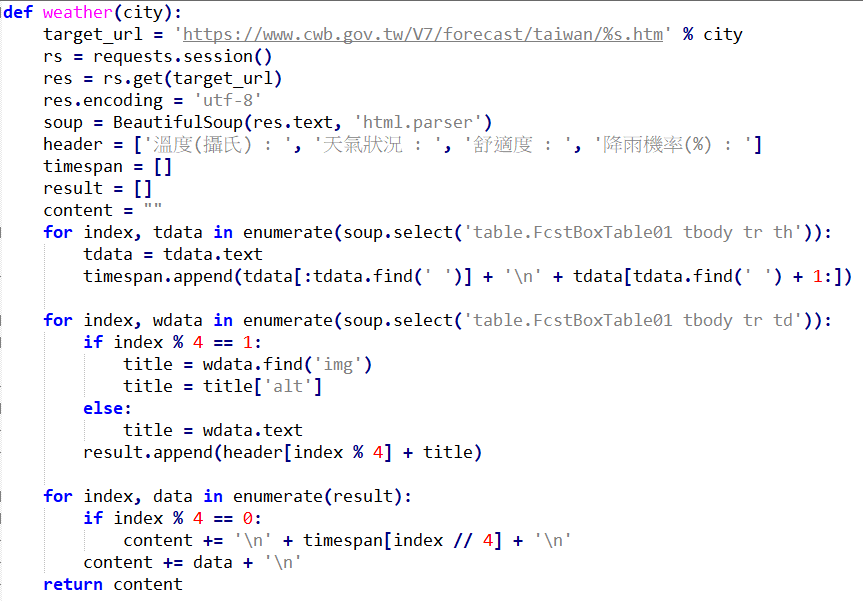
\includegraphics[width=12cm,height=8cm]{weather.png} 
\titlepage
\end{frame}

\begin{frame}%%天氣
\tikz[remember picture,overlay] \node[opacity=0.2,inner sep=0pt] at (current page.center){
\includegraphics[width=\paperwidth,height=\paperheight]{background}};
\clearpage
\frametitle{\Huge天氣 cont.}
\vspace{-1cm}
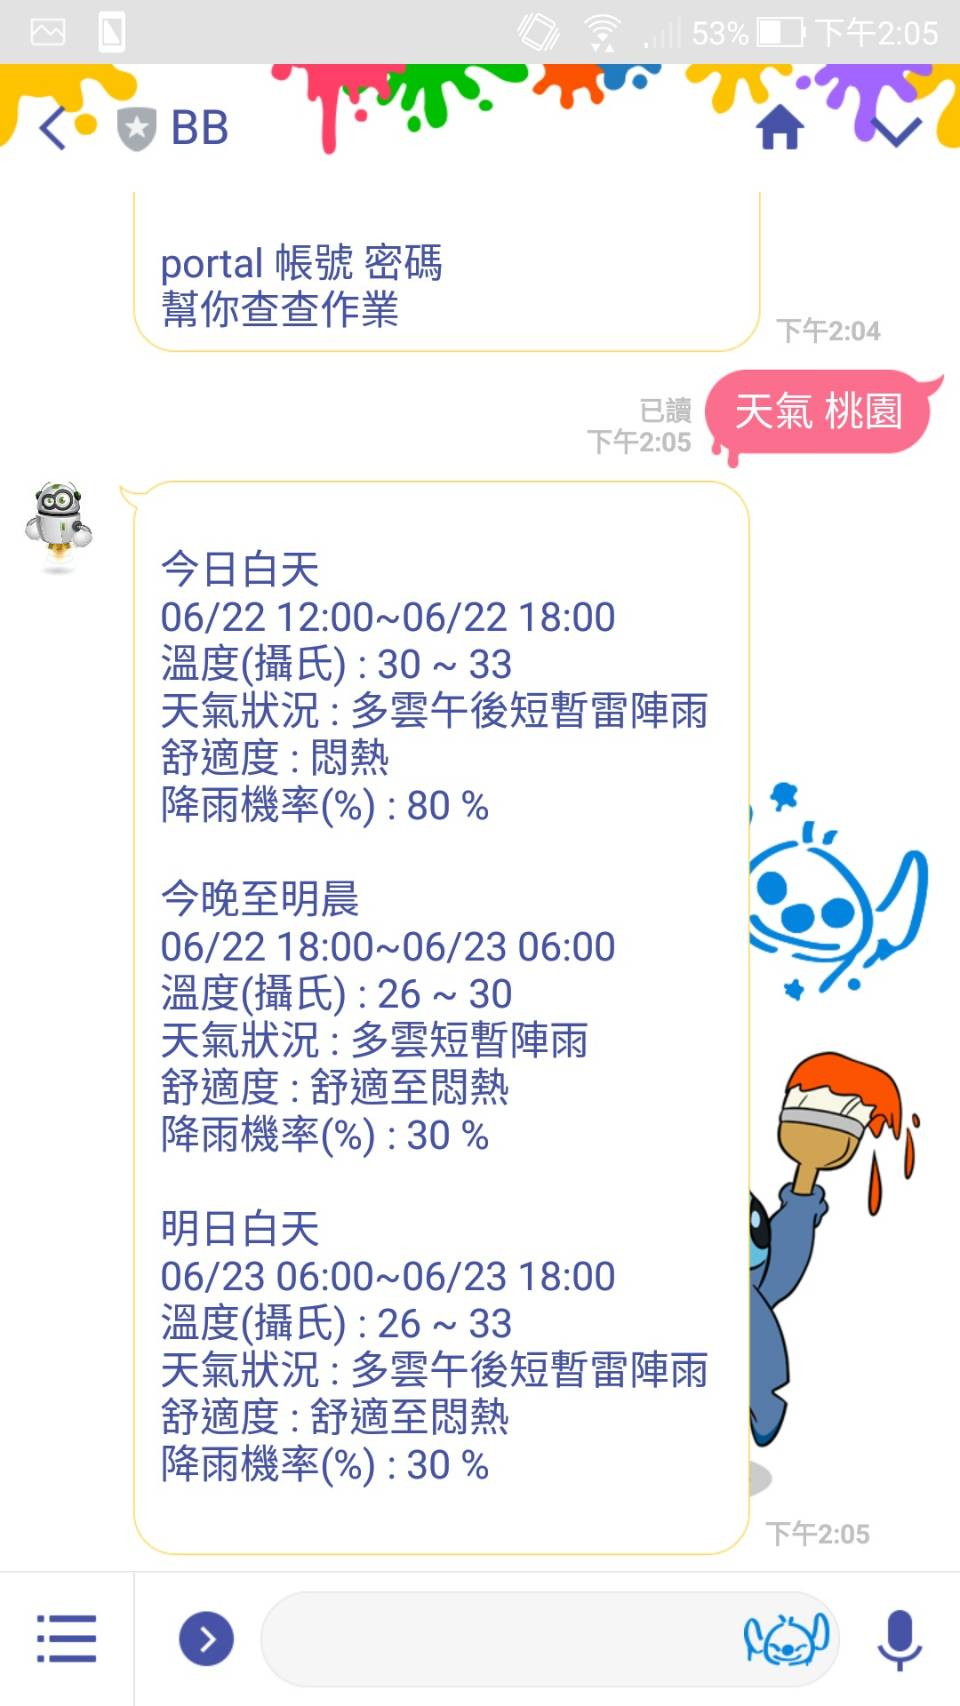
\includegraphics[width=12cm,height=8cm]{weather.jpg} 
\titlepage
\end{frame}

\begin{frame}%%YouTube
\tikz[remember picture,overlay] \node[opacity=0.2,inner sep=0pt] at (current page.center){
\includegraphics[width=\paperwidth,height=\paperheight]{background}};
\clearpage
\frametitle{\Huge YouTube}
\vspace{-1cm}
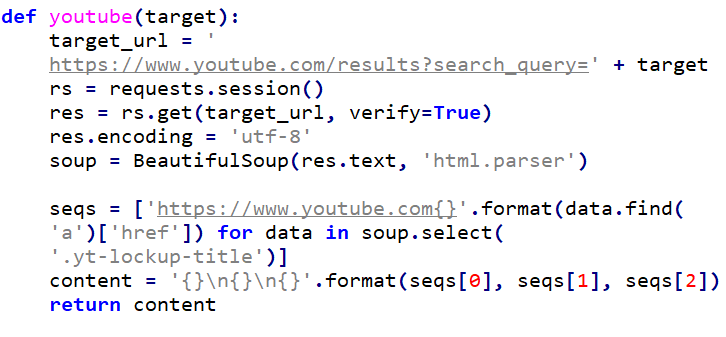
\includegraphics[width=12cm,height=8cm]{youtube.png} 
\titlepage
\end{frame}

\begin{frame}%%YouTube
\tikz[remember picture,overlay] \node[opacity=0.2,inner sep=0pt] at (current page.center){
\includegraphics[width=\paperwidth,height=\paperheight]{background}};
\clearpage
\frametitle{\Huge YouTube cont.}
\vspace{-1cm}

\includegraphics[width=12cm,height=8cm]{youtube.jpg} 
\titlepage
\end{frame}

\begin{frame}%%圖片
\tikz[remember picture,overlay] \node[opacity=0.2,inner sep=0pt] at (current page.center){
\includegraphics[width=\paperwidth,height=\paperheight]{background}};
\clearpage
\frametitle{\Huge圖片}
\vspace{-1cm}
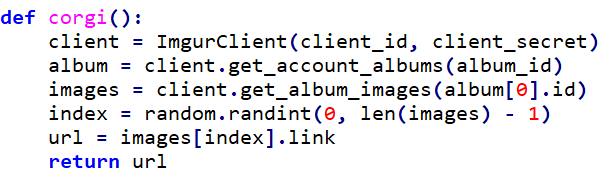
\includegraphics[width=12cm,height=8cm]{corgi.png} 
\titlepage
\end{frame}

\begin{frame}%%圖片
\tikz[remember picture,overlay] \node[opacity=0.2,inner sep=0pt] at (current page.center){
\includegraphics[width=\paperwidth,height=\paperheight]{background}};
\clearpage
\frametitle{\Huge圖片cont.}
\vspace{-1cm}

\includegraphics[width=12cm,height=8cm]{corgi.jpg} 
\titlepage
\end{frame}

\begin{frame}%%DEMO
\tikz[remember picture,overlay] \node[opacity=0.2,inner sep=0pt] at (current page.center){
\includegraphics[width=\paperwidth,height=\paperheight]{background}};
\clearpage
\title{\Huge DEMO}
\titlepage
\end{frame}

\end{CJK}
\end{document}